\section{Regkerschaltung für positive Spannugnsversorgung}
\subsection{Aufgabenstellung}
In die Anschlussklemmen des gestellten Experimentierboards ist sowohl ein LM2940 als auch ein LM7805 einzubauen. Als Last soll ein Strom von 1A bei 5V fließen dazu ist ein $R_{Last}$ zu dimensionieren. 

Von dieser Schaltung sind folgende Werte zu messen:
\begin{itemize}
    \item Spannungsrippel, Eingangsspannung an $C_1$ bei $C_1=4700\mu \text{F}$ und $C_1=1000\mu \text{F}$ und Ausgangsspannung.
    \item Minimal mögliche Eingangsspannung für den LM2940 und den LM7805.
    \item der Wirkungsgrad der beiden Regler.
\end{itemize}
\subsection{Dimensionierung}
Es soll bei einer Ausgnagsspannung von $V_{out} = 5V$ ein Strom von $I=1\rm A$ fließen. Der Widerstand R ist danach zu dimensionieren.
\begin{align}
    R&= \frac{U}{I} = \frac{5}{1} = 5\Omega \\
    P_{Dis} &= U \cdot I = 5\cdot 1 = 5 W
\end{align}
Demnach wurde ein Leistungswiderstand mit einem Wert von 5 Ohm und einer maximalen Leistungsabgabe von 15 Watt verwendet.
\subsection{Messaufbau}

\subsection{Interpretation der Messergebnisse}
\begin{figure}[H]
    \centering
    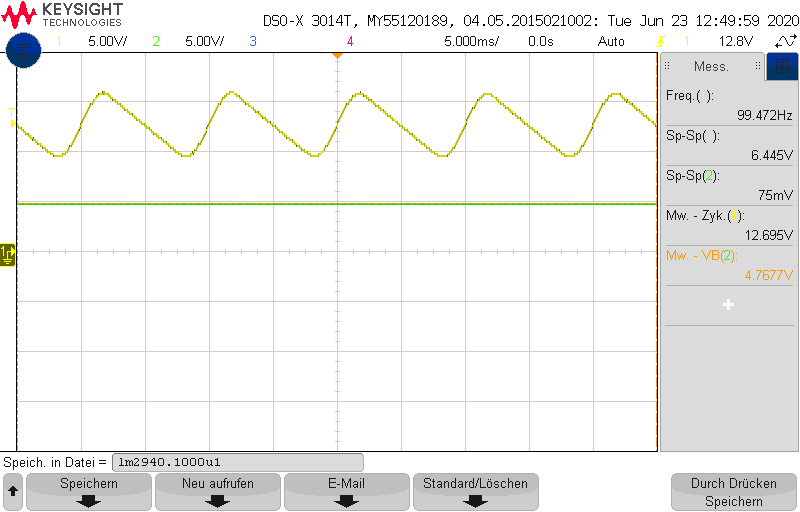
\includegraphics[width = \costumPicWidth]{Lab_5/Messungen/lm2940.1000u1.png}
    \caption{Spannungsripple LM2940, $C_1=1000\mu F$}
    \label{fig:V_rip_lm2940_1000u}
\end{figure}

\begin{figure}[H]
    \centering
    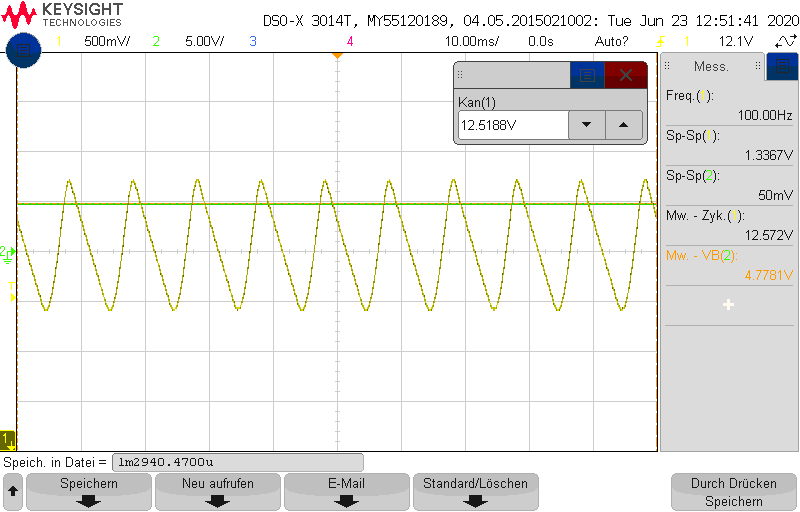
\includegraphics[width = \costumPicWidth]{Lab_5/Messungen/lm2940.4700u.png}
    \caption{Spannungsripple LM2940, $C_1=4700\mu F$}
    \label{fig:V_rip_lm2940_1000u}
\end{figure}

\begin{figure}
    \centering
    \includegraphics{}
    \caption{Spannungsripple LM7805, $C_1$}
    \label{fig:my_label}
\end{figure}
\subsection{Ausarbeitungen}
